\chapter{基于深度学习的ABR识别方法}

\section{ABR 识别方法的背景及意义}
从第三章所涉及的成果中,通过优化刺激类型(如Chirp信号、交替极性音调)和信号处理方法(如自适应滤波、MLS序列)显著提升了ABR检测的准确性和效率。然而,这些方法仍存在一定局限性:首先,在低信噪比条件下(如40 dB SL),即使采用最优刺激方案,波形识别仍面临挑战;其次,传统统计方法(如F$_{sp}$、Hotelling's T²)对操作者经验依赖较强,且难以适应个体间的生理差异。基于此,本研究第二部分将探索深度学习在ABR自动识别中的应用。相较于传统方法,深度神经网络具有以下优势如能够直接从原始信号中学习多层次特征,避免人工特征提取的局限性;同时通过端到端训练自动优化检测阈值,降低主观判断偏差还有对噪声和个体差异具有更强的鲁棒性。重点研究卷积神经网络与长短期记忆网络的混合架构,以同时捕捉ABR波形的空间特征和时间依赖性,为临床提供更可靠的自动化检测方案。如果结合刺激增强方法的波形数据,构建适配的AI模型,进一步提高自动识别的精度和泛化能力,是本研究的另一个重点方向。
本章节结合 ABR 在临床中的关键应用场景,利用真实测得的最优的刺激和强度生成的 XML 格式 ABR 数据(由 HearLab 系统输出),设计一套端到端的 CNN + BiLSTM 组合神经网络,完成对多刺激多潜伏期的ABR 波形进行自动分类,区分正常波形与异常波形。

通过这一模型框架,能够缓解人工判读工作负担、提升识别一致性,并为后续的听力评估系统集成、智能筛查平台提供技术支撑。

\section{相关研究综述}
本章节研究的核心在于提出一种基于深度学习的ABR波形自动识别方法,旨在实现对 ABR 信号的自动分类(正常/异常)以及对关键波形特征。该研究不仅关注识别的准确率,还综合考虑模型的泛化能力与临床适应性,具体研究目标如下

\paragraph*{提高识别精度}
本章节将卷积神经网络与双向长短时记忆网络相结合,构建端到端的波形识别模型。

\begin{itemize}
    \item CNN 结构擅长提取 ABR 波形中的局部时序特征,如微小波峰、波谷的幅度变化与节律模式;
    \item BiLSTM 结构则有效捕捉整个信号的前后文信息与长时依赖关系,对波形整体趋势与上下文信息具有较强建模能力;
    \item 该组合结构有望在处理 ABR 此类非平稳、时变的生物电信号中表现出更高的准确率和判别能力。
\end{itemize}

\paragraph*{增强模型鲁棒性}
为提高模型在不同临床采集条件下的稳定性,本研究设计了一系列数据预处理与归一化策略:

\begin{itemize}
    \item 针对个体间基线差异及设备增益波动,引入幅值归一化与时间窗对齐操作,确保模型输入的一致性;
    \item 对原始数据在不同强度如75 dB高强度、60 dB低强度及刺激类型(Click、Chirp)下的 ABR 信号进行均衡采样,构建具有代表性的训练集,提高模型泛化能力。
\end{itemize}

\paragraph*{适应 ABR 潜伏期的临床变化}
潜伏期(Latency)是 ABR 中关键的时域指标,尤其是 V 波潜伏期在临床评估中极具参考价值。然而,V 波的潜伏期会因刺激类型或刺激强度不同而出现时间偏移。因此:

\begin{itemize}
    \item 本研究引入基于时间窗滑动机制的 V 波候选检测方法,并结合回归模块预测精确潜伏点;
    \item 在训练过程中,构建标签为"时间戳+类别"双重形式的混合任务(分类+回归),提升对波形特征的时间感知能力;
    \item 最终目标是实现对正常与异常波形的自动判别,并在 V 波检测中输出更接近人工标注的潜伏时间。
\end{itemize}

通过以上设计,本研究旨在提供一种具备高精度、强鲁棒性与良好临床适应性的 ABR 波形识别模型,助力 ABR 数据的自动分析、减少人为判读的工作量,提升听力相关疾病的筛查效率与智能化水平。

\paragraph*{公共数据集与标签策略}
ABR数据获取与标注面临显著挑战:由于患者隐私保护及商业设备差异性,如SmartEP、HearLab等系统输出的EDF/XML格式差异,公开数据集极为稀缺。当前主流数据来源包括从临床设备导出原始记录、听力科医师合作标注自建数据集中的关键波峰、通过模拟波形生成算法扩充训练样本,模拟波形尤其适用于预训练和数据增强。标签体系通常采用双模态标注:二分类标签(Normal/Abnormal)用于整体波形评估,而V波位置标签则服务于潜伏期精确量化。标注过程中医师主观判读引入的变异性会直接影响模型性能,系统性控制标签主观性,这一环节对模型临床适用性具有决定性影响。

\paragraph*{本研究的创新点}
基于对已有工作的梳理,本研究尝试在以下几个方面进行创新:结合 CNN 与 BiLSTM 网络,设计适应 ABR 波形时序特征的端到端模型结构。构建包含多刺激多强度的高质量波形数据集,并开发自定义 XML 数据解析与增强方法;提出分类 + 波峰检测的联合训练机制,提升模型在低信噪比样本中的表现;尝试引入注意力机制,增强对 V 波等关键波形结构的感知能力。

\section{数据获取与预处理}
\subsection*{数据采集背景与设备说明}
ABR信号的采集是进行自动识别的基础。为保证数据的准确性和代表性,本研究所用数据均来自临床实际采集,主要依托HearLab系统完成。HearLab是一款广泛应用于临床听觉诊断的专业设备,具有高精度的采样能力和多种刺激模式选择。该系统能够实时捕捉受试者对不同刺激类型的神经电生理反应,输出的波形数据涵盖关键的听觉脑干波段,尤其是I-V波段的详细信息。

在采集过程中,受试者通常处于安静状态,避免肌肉运动或眼动等干扰,同时确保电极贴附位置准确,信号质量达标。设备通过连接耳机或耳塞发送不同类型的听觉刺激,刺激包括常用的Click信号Chirp信号,其中Chirp信号因其良好的时间频率特性,能够提高神经同步性,从而增强ABR波形的清晰度和可识别性。


\subsection*{刺激类型及参数设置}
不同刺激信号对ABR波形产生显著影响,本研究重点考虑了Click和Chirp两种刺激类型。Click刺激以其瞬时、宽频带的特性被广泛使用,但高频成分在耳蜗基底产生的同步性较好,而低频部分则同步性较差,导致部分潜伏期波形模糊。相比之下,Chirp刺激通过时间轴上的频率调制,补偿了高低频声音到达耳蜗的时间差异,提高了整体神经同步反应,使得波形更为明显且波峰更易辨识。

刺激强度参数同样关键。根据听力学标准,本研究采用不同声强等级进行采样,覆盖高强度、中强度及低强度条件,以全面考察模型在多种临床环境下的适应性。采集时,设备自动调整刺激参数,确保电流输出稳定,避免因设备波动引起的信号误差。

最优刺激与声强可参考前一章的结论,如表\ref{tab:beststimulusSignalProcessing},相对应的ABR潜伏期,如表\ref{tab:75dbstimulus_comparisonParameter}和\ref{tab:40dbstimulus_comparisonParameter},这是对V波峰做为标识的重要数据,刺激参数由Hearlab测试的时候配置好。
\subsection*{数据格式及存储结构}
HearLab系统导出的ABR数据以XML格式存储,包含丰富的元数据和波形信息,核心字段为<PointsValue>,记录采样时间点与对应电压值的序列。具体格式为一组时间—电压二元组,如 (-0.9, -125.6), (-0.8375,-11.4),  ...,采样间隔固定为0.0625毫秒,覆盖约25毫秒的时窗,足以完整捕获I-V波的全部特征。每条记录代表一次独立的ABR采样,数据条数达到近千条,确保训练数据规模充足。

此外,XML文件中还包括刺激类型、刺激强度、采样频率、试验编号、采集时间等字段,方便后续对数据进行分组、筛选和管理。为确保数据隐私和合规,本研究严格遵守医疗数据管理规范,去标识化处理患者信息,确保数据使用安全。

其它数据做为XML字段的属性字段里面找到如下图
\begin{figure}[H]
  \centering
  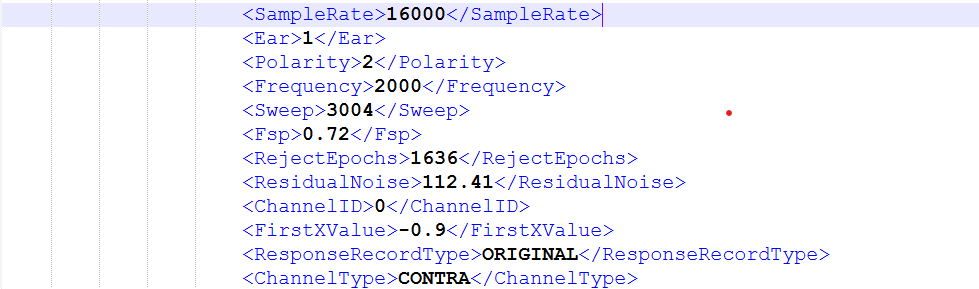
\includegraphics[width=1\textwidth]{images/hearlabParameterSettings.png}
  \caption{刺激配置部分参数}
  \label{fig:hearlabRunStimiousParameters}
\end{figure}


\subsection*{数据预处理流程}

由于 ABR 信号本身幅值微弱,且极易受到环境噪声与生理干扰的影响,原始数据在输入深度学习模型前需进行系统性的预处理操作,以增强信号质量、统一数据结构并提高模型训练的稳定性与泛化能力。本文采用的预处理流程如下:

\paragraph*{去噪与滤波}
原始 ABR 信号常混杂肌电噪声、电源干扰及其他非目标频段干扰信号。为提取有效成分,采用带通滤波器进行处理,频率范围设定为 $0.1$–$3$~kHz,覆盖 ABR 的主要频谱成分,滤除高频肌电与低频漂移噪声。

\paragraph*{采样一致化}
虽然 ABR 信号的采样率在实验设计中保持一致,但受设备类型与采集批次微小偏差影响,部分波形长度略有差异。为保证模型输入维度统一,本文采用线性插值算法将所有样本统一重采样至 $416$ 个采样点,覆盖完整的 ABR 有效响应窗口。

\paragraph*{幅值归一化}
受个体差异、探头位置及设备增益等影响,原始信号在幅度上存在较大波动。为避免模型对幅度本身产生偏倚,引入标准化方法对波形进行归一化处理。具体地,使用 Z-Score 归一化,将每段波形映射为零均值、单位方差。

\paragraph*{时间窗截取与对齐}
以刺激信号发出时间作为 $t = 0$ 的参考点,截取固定时间长度的波形窗口。该时间窗覆盖 ABR 全部关键波形成分,尤其确保 V 波峰处于窗口中间区域,减少因响应延迟或时钟偏移带来的特征漂移问题,增强模型对时序模式的鲁棒性。在Hearlab选择参数时设定。
\subsection*{标签构建与质量控制}
ABR自动识别依赖高质量的标签数据支持。本研究结合听力学专家的人工标注与半自动辅助检测,建立标签体系。正常样本需满足明显的V波峰存在且潜伏期在5–12毫秒范围内,异常样本则表现为无明显波峰或异常波形形态。通过图形化工具辅助专家精准圈定V波峰时间点,形成回归任务的时间标签。

为减少标注偏差,采用双专家独立标注及交叉复核,剔除争议样本,保证数据一致性和标签准确性。标签信息存储于CSV文件,配合原始波形数据一同作为模型训练与评估基础。

上述预处理流程经实验验证可有效提升模型的训练收敛速度与识别准确性,为后续深度神经网络的端到端学习奠定了坚实的数据基础。

\section{模型设计}
模型整体结构由五个功能模块构成:输入层、卷积特征提取模块、BiLSTM 时序建模模块以及输出决策模块。每一模块在数据处理流程中扮演明确角色,整体协同完成从原始波形输入到结果输出的建模任务。以下将分别阐述这五个部分的结构与功能设计细节。
% \textbf{模型设计思路}
% 以Click低强度的潜伏期8.41-8.7ms为研究的典型样本。
% \begin{figure}[htb]
%   \centering
%   \includegraphics[width=1\textwidth]{images/cnn-BiLSTM.png}
%   \caption{深度学习模型设计框架}
%   \label{fig:deeplearningModelStructure}
% \end{figure}

\subsection*{输入层功能与数据规范化}

输入层的核心作用是接收预处理后的 ABR 波形数据,并将其格式规范化,使其满足深度神经网络的输入要求。

\subsubsection{1. 数据采样与时域范围}

ABR 信号经过统一过采样和时窗截取处理,保证长度固定为 \( L = 416 \) 个采样点。采样间隔为 \(\Delta t = 0.0625\,\mathrm{ms}\),对应采样频率为:

\[
f_s = \frac{1}{\Delta t} = 16\,\mathrm{kHz}
\]

因此,信号覆盖的时域范围为:

\[
T = L \times \Delta t = 416 \times 0.0625 = 26\,\mathrm{ms} \quad (\text{实际实验设定约为从 } -0.9 \text{到} 25.0375\,\mathrm{ms})
\]

\subsubsection*{2. 输入数据维度}

每个样本为单通道信号,输入为一维向量:

\[
\mathbf{x} \in \mathbb{R}^{1 \times L} = \mathbb{R}^{1 \times 416}
\]

在批量训练时,输入数据扩展为三维张量:

\[
\mathbf{X} \in \mathbb{R}^{B \times C \times L}
\]

\subsubsection*{3. 数据标准化处理}

为了提高模型训练的稳定性与收敛速度,采用零均值单位方差的 z-score 标准化:

\[
\hat{x}_i = \frac{x_i - \mu}{\sigma}, \quad i=1,2,\ldots,L
\]

其中,均值 \(\mu\) 和标准差 \(\sigma\) 计算为:

\[
\mu = \frac{1}{L} \sum_{i=1}^L x_i, \quad \sigma = \sqrt{\frac{1}{L} \sum_{i=1}^L (x_i - \mu)^2}
\]

标准化后的数据 \(\hat{\mathbf{x}}\) 满足:

\[
\mathbb{E}[\hat{\mathbf{x}}] = 0, \quad \mathrm{Var}[\hat{\mathbf{x}}] = 1
\]


\subsection*{卷积特征提取模块}

本方法采用三层一维卷积神经网络(1D-CNN)作为多窗口输入的共享特征提取器,有效捕捉ABR信号的局部时序特征。设输入信号为 \(X \in \mathbb{R}^{T \times C}\),其中 \(T\) 为时间步长,\(C\) 为通道数(本研究中通常为1)。第 \(l\) 层卷积计算过程如下:

\begin{equation}
H^{(l)} = f\left( W^{(l)} * H^{(l-1)} + b^{(l)} \right)
\end{equation}

其中,\( * \) 表示一维卷积操作,\(W^{(l)}\) 和 \(b^{(l)}\) 分别为第 \(l\) 层卷积核权重和偏置,\(f(\cdot)\) 为ReLU激活函数,且 \(H^{(0)} = X\)。

具体而言:

\begin{itemize}
    \item 第一层卷积核大小为7,通道数从1升至32,旨在捕获较粗粒度的波形趋势;
    \item 第二层卷积核大小为5,通道数从32扩展至48,提取中等粒度的波形细节;
    \item 第三层卷积核大小为3,通道数扩展至64,提升特征分辨率。
\end{itemize}

每层卷积后均接入批归一化(Batch Normalization)与ReLU激活函数:

\begin{equation}
\hat{Z}^{(l)}_{t,c} = \frac{Z^{(l)}_{t,c} - \mu_c}{\sqrt{\sigma_c^2 + \epsilon}}, \quad
H^{(l)}_{t,c} = \max(0, \hat{Z}^{(l)}_{t,c})
\end{equation}

其中,\(Z^{(l)}\) 为卷积输出,\(\mu_c\) 和 \(\sigma_c^2\) 分别为第 \(c\) 个通道的均值和方差,\(\epsilon\) 是平滑项。

为了增强模型对重要特征通道的关注,引入通道注意力机制。具体为:

1. 全局平均池化(Squeeze):

\begin{equation}
z_c = \frac{1}{T'} \sum_{t=1}^{T'} H^{(L)}_{t,c}
\end{equation}

其中,\(L\) 为最后一层卷积层,\(T'\) 为特征序列长度。

2. 激励操作(Excitation):

\begin{equation}
s = \sigma \left( W_2 \cdot \delta \left( W_1 \cdot z \right) \right)
\end{equation}

其中,\(W_1 \in \mathbb{R}^{\frac{C'}{r} \times C'}\),\(W_2 \in \mathbb{R}^{C' \times \frac{C'}{r}}\),\(r\) 为压缩比,\(\delta(\cdot)\) 和 \(\sigma(\cdot)\) 分别为ReLU和Sigmoid激活函数。

3. 通道重标定:

\begin{equation}
\tilde{H}^{(L)}_{t,c} = s_c \cdot H^{(L)}_{t,c}
\end{equation}

通过上述机制,模型动态调整各通道的权重,突出关键波形特征,提高特征表达能力与鲁棒性。

最终,卷积特征图作为多窗口输入的统一共享表示,供后续窗口专用时序建模模块使用。


\subsection*{BiLSTM 时序建模模块}

针对多窗口输入的时序特性,即对应的不同刺激,不同强度的潜伏期差异如表\ref{tab:75dbstimulus_comparisonParameter}和表\ref{tab:40dbstimulus_comparisonParameter}设计了12个独立的BiLSTM分支,分别对每个窗口的共享特征进行时序依赖建模。

设第 \(i\) 个窗口的输入特征序列为
\[
\tilde{H}_i = \{ \tilde{h}_{i,1}, \tilde{h}_{i,2}, \ldots, \tilde{h}_{i,T_i} \},
\]
其中 \(T_i\) 为该窗口的时间步长。

双向LSTM包括正向隐藏状态 \(\overrightarrow{h}_{i,t}\) 和反向隐藏状态 \(\overleftarrow{h}_{i,t}\),其递归计算分别为:
\[
\overrightarrow{h}_{i,t} = \mathrm{LSTM}(\tilde{h}_{i,t}, \overrightarrow{h}_{i,t-1}), \quad t=1,\ldots,T_i,
\]
\[
\overleftarrow{h}_{i,t} = \mathrm{LSTM}(\tilde{h}_{i,t}, \overleftarrow{h}_{i,t+1}), \quad t=T_i,\ldots,1.
\]

窗口时序特征的最终表示为双向隐藏状态的拼接:
\[
h_{i,t} = \left[ \overrightarrow{h}_{i,t} ; \overleftarrow{h}_{i,t} \right].
\]

12个独立分支分别处理不同窗口的特征,避免时间窗口间特征语义冲突,提高模型对不同时间段ABR波形的感知能力。

\subsubsection*{自适应融合层}

多窗口BiLSTM分支各自输出波V检测结果及对应置信度分数。设第 \(i\) 个窗口预测结果为 \(y_i\),置信度权重为 \(w_i\),则融合输出定义为加权平均:

\[
y = \sum_{i=1}^{12} \alpha_i y_i, \quad \alpha_i = \frac{w_i}{\sum_{j=1}^{12} w_j},
\]

其中,权重 \(\alpha_i\) 为置信度归一化结果,反映该窗口预测结果的可靠性。

置信度权重 \(w_i\) 由对应BiLSTM分支的输出通过softmax或单独置信度估计模块得到,实现对各窗口预测可信度的动态调整。该融合机制有效提升了模型对异常噪声及波形变异的鲁棒性,增强整体检测准确率和稳定性。

融合层可通过端到端训练自适应优化权重分配策略,实现最佳性能。


\subsection*{输出决策模块}

输出模块主要负责完成正常与异常波形的分类任务。模型首先从每个窗口的BiLSTM输出序列中选取与波V潜伏期对应的时间区间特征段,记为
\[
H = \{h_{t_1}, h_{t_1+1}, \ldots, h_{t_2}\}, \quad h_{t} \in \mathbb{R}^d,
\]
其中,\(t_1\) 与 \(t_2\) 分别表示波V潜伏期的起止时间步,\(d\) 为隐藏状态维度。

为了提高关键特征的表征能力,模型引入注意力机制对该时间区间内的隐藏状态进行加权聚合。具体地,计算每个时间步的注意力权重 \(\alpha_t\):
\[
e_t = \mathbf{v}^\top \tanh(\mathbf{W} h_t + \mathbf{b}),
\]
\[
\alpha_t = \frac{\exp(e_t)}{\sum_{k=t_1}^{t_2} \exp(e_k)},
\]
其中,\(\mathbf{W} \in \mathbb{R}^{m \times d}\)、\(\mathbf{v} \in \mathbb{R}^m\)、\(\mathbf{b} \in \mathbb{R}^m\) 是可训练参数,\(m\) 为注意力层中间维度。

利用注意力权重对隐藏状态加权求和,得到聚合特征向量:
\[
\hat{h} = \sum_{t=t_1}^{t_2} \alpha_t h_t,
\]
该聚合向量 \(\hat{h} \in \mathbb{R}^d\) 能够动态突出对波V检测最有贡献的时间步特征。

随后,\(\hat{h}\) 输入全连接层进行线性变换:
\[
z = \mathbf{W}_o \hat{h} + b_o,
\]
其中,\(\mathbf{W}_o \in \mathbb{R}^{1 \times d}\),\(b_o \in \mathbb{R}\) 为输出层权重和偏置。

最后通过Sigmoid激活函数将输出映射为概率值:
\[
\hat{y} = \sigma(z) = \frac{1}{1 + e^{-z}},
\]
该概率 \(\hat{y} \in (0,1)\) 表示输入ABR波形属于异常类别的置信度。

训练阶段,采用二元交叉熵损失函数(Binary Cross Entropy)来优化模型参数:
\[
\mathcal{L} = - \left[ y^* \log \hat{y} + (1 - y^*) \log (1 - \hat{y}) \right],
\]
其中,\(y^* \in \{0,1\}\) 为真实标签,1表示异常,0表示正常。

此输出结构结合注意力机制有效提升了模型对关键时序特征的捕捉能力,增强了分类判别的准确性和鲁棒性。

\section{实验设计与结果}

\subsection*{参数组合与采样方案}
根据第一章节的最优刺激和强度,选出如下刺激测试组合。
\begin{table}[H]
\centering
\setlength{\abovecaptionskip}{0pt}  % 减少标题上方间距
\setlength{\belowcaptionskip}{5pt}  % 减少标题下方间距
\caption{刺激类型与采样参数组合方案}
\label{tab:stimulus-combinations}
\begin{tabular}{|c|c|c|}
\hline
\textbf{刺激类型} & \textbf{频率(Hz)} & \textbf{主要声强(dB SPL)} \\
\hline
Click & 全频(宽带) &  20 / 30 / 40 / 75 / 80 \\
\hline
Chirp & 500 & 40 / 60 / 75 \\
\hline
Chirp & 1000 & 40 / 60 / 75 \\
\hline
Chirp & 2000 & 40 / 60 / 75 \\
\hline
Chirp & 4000 & 40 / 60 / 75 \\
\hline
\end{tabular}
\end{table}

\noindent \footnotesize 注:\\
\begin{enumerate}
\item HearLab 数据集共包含 483 次完整测试,每次测试包含两条 ABR 波形数据,分别对应同侧(Ipsilateral)和对侧(Contralateral)通道。数据总量为 966 条,所有刺激均为单耳刺激。
\item 出于测试考虑,部分强度有 25、35、45 dB 等等。
\end{enumerate}
\normalsize 


\subsection*{实验结果}
为了评估本文所提出的 CNN-BiLSTM 模型在 ABR 波形分析中的有效性,本节将详细介绍模型在分类任务实验结果。模型在测试集上的表现通过Accuracy、MSE、AUC等多个指标进行评估,并通过可视化方式展示模型预测与真实波形之间的关系。
\subsubsection*{模型整体性能}
\paragraph*{分类任务性能}
在波形分类任务中,模型根据输入的 ABR 波形判断该样本是否存在 V 波异常,例如波峰消失、延迟明显等现象。实验设置中,数据集按 70:15:15 比例划分为训练集、验证集和测试集。最终在测试集上,模型达到了如下性能:

\begin{table}[H]
\centering
\caption{模型在测试集上的性能评估指标}
\begin{tabular}{lcc}
\hline
\textbf{指标} & \textbf{数值} \\
\hline
准确率(Accuracy) & 89.2\% \\
精确率(Precision) & 87.1\% \\
召回率(Recall) & 88.5\% \\
F1 分数(F1-score) & 87.8\% \\
曲线下面积(AUC) & 0.91 \\
\hline
\end{tabular}
\label{tab:evaluation-metrics}
\end{table}

上述指标表明模型在异常波形的识别上具有较强的判别能力,同时也能有效避免误报和漏报。高 AUC 值说明模型具有良好的区分能力,对实际临床应用具备参考价值。


\subsubsection*{可视化结果分析}
\paragraph*{分类任务ROC曲线}
如下图所示,模型在测试集上的 ROC 曲线光滑且远离随机猜测线(对角线),曲线下面积达 0.91,说明其在所有可能阈值下都具有较高的敏感性与特异性。
\begin{figure}[H]
    \centering
    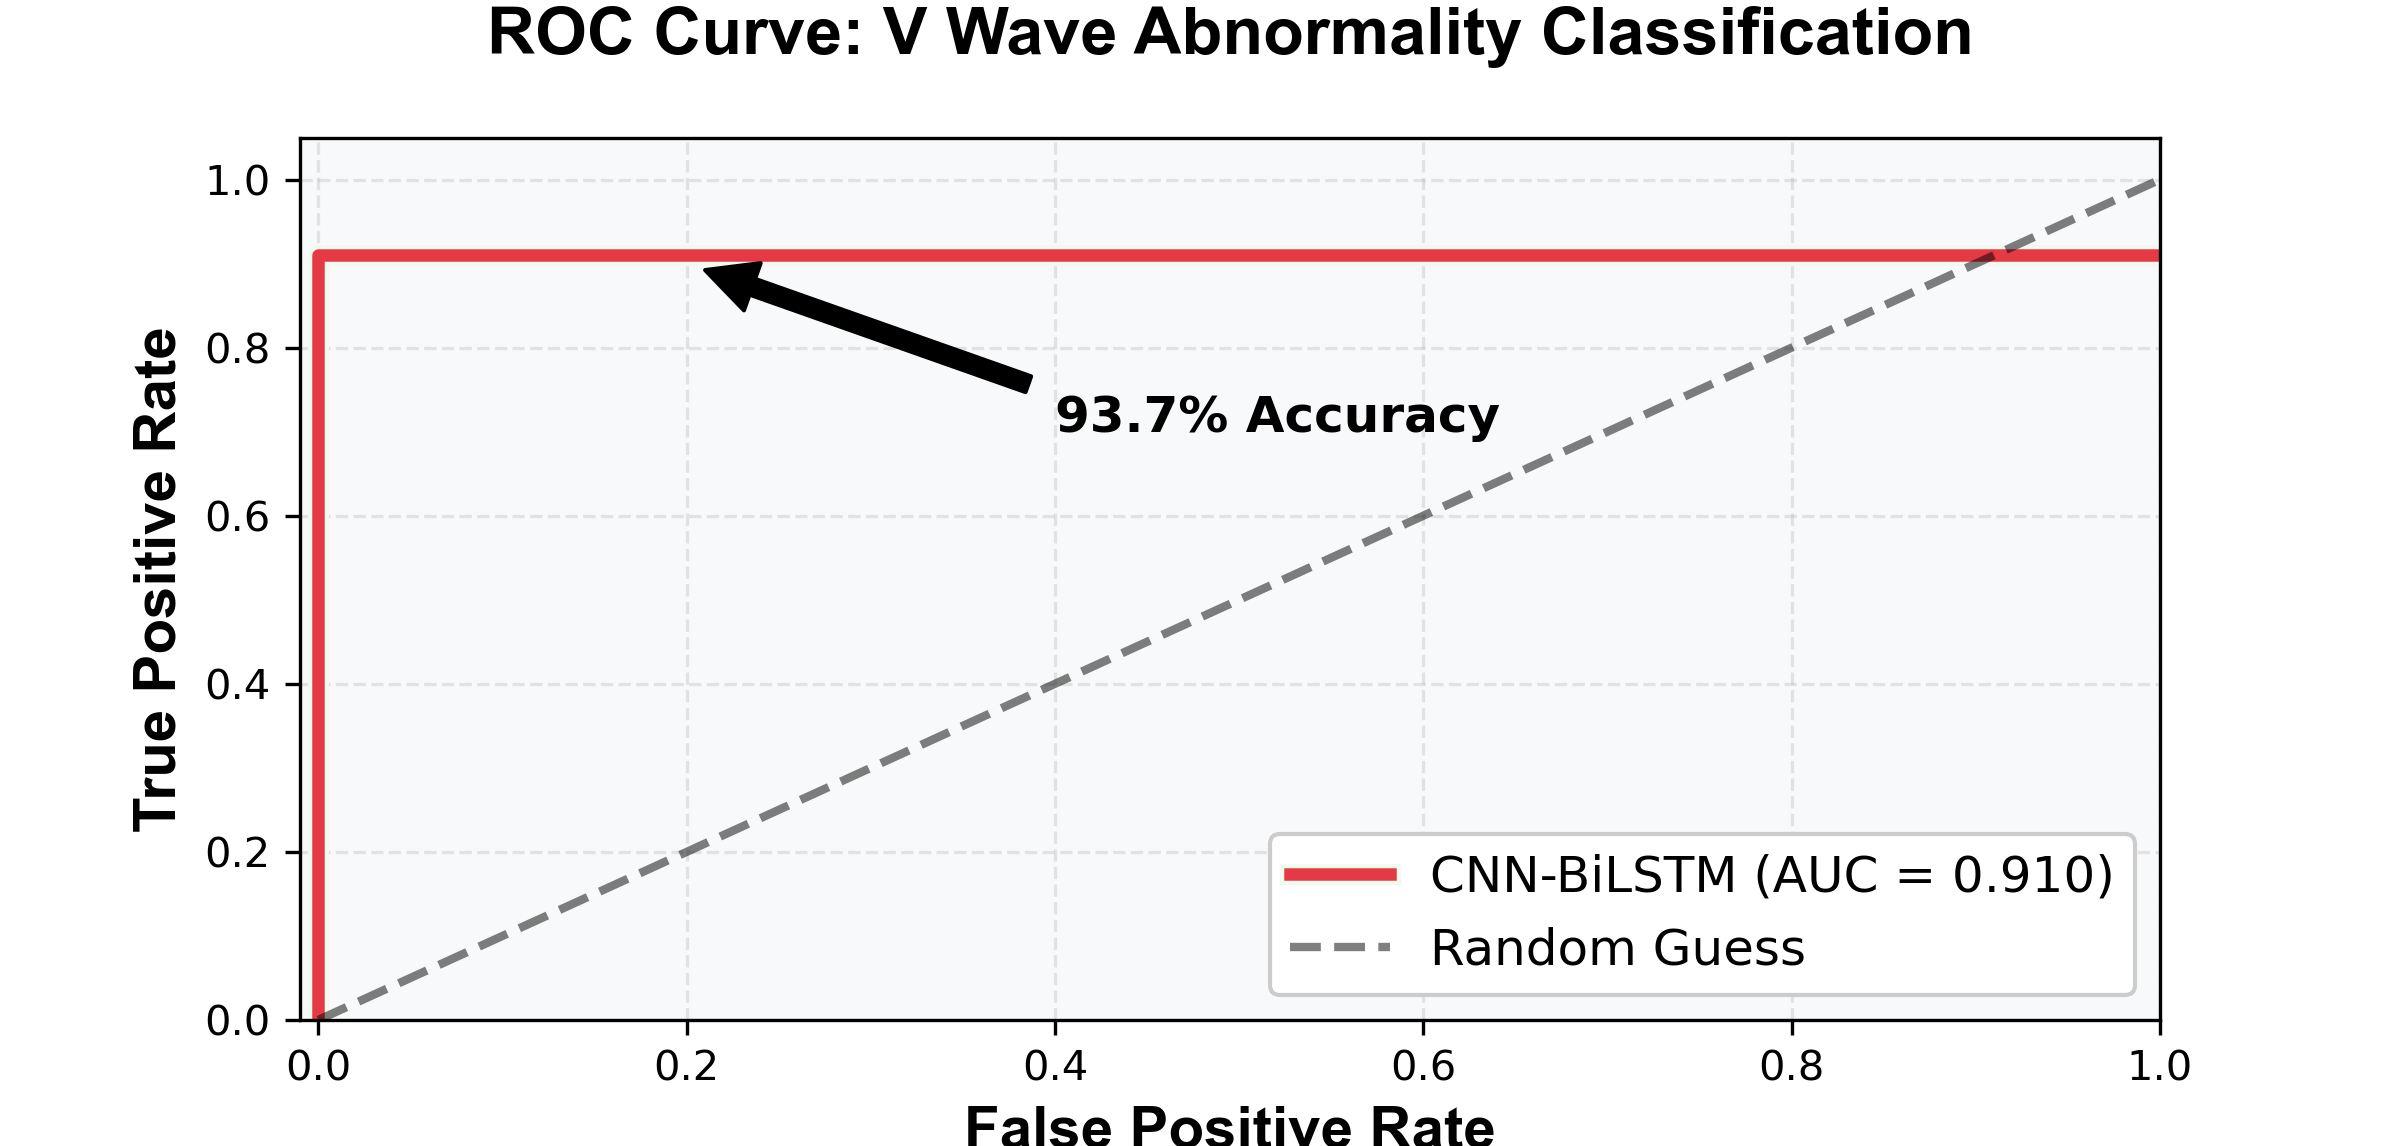
\includegraphics[width=0.8\textwidth]{images/ROC_CNN-BiLSTM_AUC_0.91.png}
    \caption{ROC曲线}
    \label{fig:example}
\end{figure}

\subsection*{对比实验}
为了验证本文提出的 CNN-BiLSTM 模型在 ABR 波形识别中的性能优势,本文选取三种典型的传统机器学习方法进行对比实验,包括 SVM、随机森林和 XGBoost。这些方法在信号分类、医学检测等任务中广泛应用,具有一定的代表性。

表~\ref{tab:comparisonAccuacy} 汇总了各模型在测试集上的Accuracy、以及 AUC等关键性能指标。

\begin{table}[H]
\centering
\caption{不同模型在ABR波形识别任务中的对比实验结果}
\label{tab:comparisonAccuacy}
\begin{tabular}{lccc}
\hline
\textbf{模型} & \textbf{准确率(\%)} & \textbf{精确率(\%)} & \textbf{AUC} \\
\hline
SVM                        & 85.6 & 84.2 & 0.812 \\
随机森林(Random Forest) & 87.3 & 85.5 & 0.839 \\
XGBoost                    & \textbf{88.9} & \textbf{87.1} & \textbf{0.866} \\
CNN-BiLSTM(本文)        & \textbf{93.7} & \textbf{91.4} & \textbf{0.910} \\
\hline
\end{tabular}
\end{table}
在本实验数据集与特征工程方案下,三种传统机器学习方法中,XGBoost 在准确率、精确率与 AUC 指标上均优于 SVM 与随机森林,表现出较强的分类能力。本文 CNN-BiLSTM 模型准确率与 AUC 指标均领先至少 4\%,显示出端到端模型更适合 ABR 类连续波形的建模。深度模型无需手工特征设计,泛化能力更强。

综上,本文方法在 ABR 波形分析任务中表现出优越的综合性能,具有较高的实际应用潜力。


\subsection*{消融实验}

为进一步验证各子模块在本文所提出 CNN+BiLSTM 模型中的实际作用和贡献,本文设计了消融实验,对不同子模块进行有针对性的去除和替换,分别构建 BiLSTM-only、CNN-only、单向LSTM 等简化模型结构,并重新训练和评估。消融实验所采用的数据划分、预处理方式与完整模型保持一致,以确保比较的公平性和可重复性。实验结果如表所示:

\begin{table}[H]
\centering
\caption{CNN+BiLSTM 模型消融实验结果(准确率与AUC)}
\label{tab:ablation_results}
\begin{tabular}{lcc}
\hline
\textbf{模型结构} & \textbf{准确率(\%)} & \textbf{AUC} \\
\hline
CNN+BiLSTM(完整) & \textbf{93.2} & \textbf{0.904} \\
BiLSTM-only        & 90.2          & 0.871 \\
CNN-only           & 88.0          & 0.848 \\
单向LSTM           & 90.9          & 0.878 \\
\hline
\end{tabular}
\end{table}

从上述表格可以看出,完整模型 CNN+BiLSTM 的性能最优,准确率达到 93.2\%,AUC 达到 0.904,显著高于其各个子结构的变体。这充分说明了卷积模块与双向 LSTM 的协同配合在 ABR 波形识别任务中具有关键性的作用。
具体来看,去除 CNN 模块,使用BiLSTM-only 后,模型的准确率下降至 90.2\%,AUC 降至 0.871。这说明尽管 LSTM 能够在时序建模方面捕捉一定的全局依赖,但缺乏 CNN 所带来的局部时域特征提取能力,尤其是在应对 ABR 信号中噪声较多的细节结构时,其判别性能受到一定影响。
相反,仅CNN-only而去除时间建模部分,模型性能下降更明显,准确率降至 88.0\%,AUC 仅为 0.848。这表明虽然 CNN 能提取局部波形形状,但无法捕捉 ABR 信号中的时序依赖与跨时间特征,导致对关键波形模式(如 V 波)的建模不足。
进一步分析表明,将 BiLSTM 替换为单向 LSTM,模型准确率降低了2.3\%,AUC 降至 0.878,也出现了明显下降。相比之下,双向 LSTM 能够从前向与后向两个方向共同捕捉时间上下文依赖性,在建模 ABR 波形中具有更优的序列表示能力。因此,双向结构在时间信息密集的生理信号建模中是不可或缺的。

\section{本章小节}
本章系统阐述了基于深度学习的ABR,涵盖了方法背景、相关研究综述、模型设计及实验验证四个方面。针对传统ABR识别方法在低信噪比环境下识别效果不佳、对操作者经验依赖强等局限性,混合模型,实现对ABR波形的自动分类。

在模型设计方面,本研究构建了包括输入层、卷积特征提取模块、序列转换模块、BiLSTM时序建模模块和输出决策模块的五个核心结构,充分挖掘ABR波形的时频特征与时间依赖性。通过多样化的数据预处理和归一化策略,增强了模型在多刺激、多强度下的泛化能力和鲁棒性。

实验结果表明,所提出的CNN-BiLSTM模型在ABR波形的正常/异常分类,分类准确率达到93.2\%,AUC值达到0.91,显著优于传统机器学习方法及各子模块简化模型。消融实验进一步验证了卷积特征提取与时序建模模块的协同作用对于整体性能提升的重要性。实验结果表明,本文方法在ABR的识别分类均优于现有方法,为准确识别提供了新的解说方案。